\documentclass[12pt,a4paper]{article}

\usepackage{fontspec}
\usepackage{polyglossia}
\setdefaultlanguage{russian}
\setmainfont{Times New Roman}
\newfontfamily\cyrillicfont{Times New Roman}
\newfontfamily\cyrillicfontsf{Times New Roman}
\newfontfamily\cyrillicfonttt{Courier New}
\setmonofont{Courier New}
\usepackage{amsmath,amssymb,mathtools}
\usepackage{geometry}
\usepackage{hyperref}
\usepackage{xcolor}
\usepackage{listings}
\usepackage{booktabs}
\usepackage{graphicx}
\usepackage{float}
\usepackage{caption}
\usepackage{enumitem}

\geometry{left=25mm,right=20mm,top=20mm,bottom=25mm}
\captionsetup{font=small,labelfont=bf,skip=6pt}
\setlist{nosep,leftmargin=*}

\hypersetup{colorlinks=true,linkcolor=blue,urlcolor=blue}

\lstdefinelanguage{JavaScript}{
  keywords={const,let,var,function,return,if,else,for,while,import,from,export,
            default,new,class,throw,true,false,null,undefined,Math,Array},
  sensitive=true,
  comment=[l]{//},
  morecomment=[s]{/*}{*/},
  morestring=[b]", morestring=[b]', morestring=[b]`
}

\lstdefinestyle{jsstyle}{
  basicstyle=\ttfamily\small,
  breaklines=true,
  frame=single,
  columns=fullflexible,
  keepspaces=true,
  showstringspaces=false,
  keywordstyle=\color{blue!60!black},
  commentstyle=\color{green!40!black},
  stringstyle=\color{red!50!black}
}
\lstset{style=jsstyle}

\begin{document}

\begin{titlepage}
  \centering
  \vspace*{1.5cm}

  {\Large Отчёт по вычислительному практикуму\par}
  \vspace{2.5cm}

  {\LARGE\bfseries Модуль «Магнитные колебания»\par}
  \vspace{1cm}

  {\Large Задача 4. Связанные маятники\par}

  \vfill

  \begin{flushright}
    \begin{minipage}{0.55\textwidth}
      \raggedleft
      Выполнил:\\
      студент группы M3203\\
      Георгий Габатов\\[12pt]
      Преподаватель:\\
      Шоев~И.~В.
    \end{minipage}
  \end{flushright}

  \vspace{2cm}

  {\large Санкт-Петербург\\[6pt]
  \the\year\par}

\end{titlepage}

\begin{abstract}
\noindent
В работе построена компьютерная модель двух связанных математических маятников
с вязким затуханием. Выведены уравнения движения при малых углах, найдены
нормальные частоты, реализовано численное интегрирование методом Рунге-Кутты
4-го порядка. Интерактивное демо позволяет изменять параметры модели и
наблюдать биения, затухание и влияние жёсткости пружины. Численные результаты
согласованы с аналитическими формулами и спектральным анализом (погрешность
определения частот менее 2\%).
\end{abstract}

\tableofcontents
\newpage

%======================================================================
\section{Цель и постановка задачи}
%======================================================================

\subsection{Формулировка из задания}

Даны два одинаковых математических маятника, связанных пружиной с коэффициентом
жёсткости \(k\). Точка крепления пружины находится на расстоянии \(L_1\) от точки
подвеса каждого маятника. Точки крепления обоих маятников расположены на одном
уровне. Маятники имеют одинаковые длину подвеса \(L\), массу \(m\). Сила
сопротивления каждого маятника прямо пропорциональна скорости, коэффициент
затухания --- \(\beta\).

\textbf{Требуется:}
\begin{enumerate}
  \item для заданных начальных отклонений построить графики зависимостей
        углов и скоростей от времени для каждого маятника;
  \item найти нормальные частоты;
  \item обеспечить возможность задания параметров пользователем.
\end{enumerate}

\subsection{Цель работы}

Цель --- не только получить конкретные графики при одном наборе параметров, но и:
\begin{itemize}
  \item обосновать выбор математической модели и явно указать допущения;
  \item вывести уравнения движения из законов Ньютона;
  \item реализовать устойчивый численный метод интегрирования ОДУ;
  \item проверить корректность по аналитическим асимптотикам и автотестам;
  \item исследовать влияние параметров (\(k\), \(\beta\), начальные условия)
        на характер колебаний.
\end{itemize}

%======================================================================
\section{Физическая модель}
%======================================================================

\subsection{Геометрия системы}

Рассматривается следующая конфигурация:
\begin{itemize}
  \item два математических маятника подвешены на одной горизонтальной линии;
  \item каждый маятник --- материальная точка массы \(m\) на невесомом стержне
        длины \(L\);
  \item горизонтальная пружина жёсткости \(k\) соединяет точки на стержнях,
        отстоящие на \(L_1\) от осей подвеса;
  \item в равновесии (\(\theta_1=\theta_2=0\)) пружина не деформирована.
\end{itemize}

При отклонении первого маятника на угол \(\theta_1\) точка крепления пружины
смещается горизонтально примерно на \(L_1\sin\theta_1\approx L_1\theta_1\)
(при малых углах). Аналогично для второго маятника. Разность смещений определяет
растяжение пружины.

\subsection{Допущения модели}

\begin{table}[H]
\centering
\caption{Допущения и их физический смысл}
\begin{tabular}{@{}p{4.2cm}p{9.5cm}@{}}
\toprule
Допущение & Обоснование \\
\midrule
Малые углы: \(\sin\theta\approx\theta\) &
  Линейная модель; при \(\theta\gtrsim15^\circ\) нужна нелинейная теория \\[4pt]
Пружина горизонтальна &
  При малых \(\theta\) вертикальное смещение точки крепления
  \(L_1(1-\cos\theta)\approx L_1\theta^2/2\) пренебрежимо мало \\[4pt]
Стержни невесомы &
  Момент инерции \(I=mL^2\) \\[4pt]
Вязкое затухание: \(F=-\beta v\) &
  Линейная модель сопротивления воздуха при малых скоростях \\[4pt]
Пружина без массы &
  Мгновенная передача силы \\
\bottomrule
\end{tabular}
\end{table}

\subsection{Вывод уравнений движения}

\paragraph{Шаг 1. Смещение точки крепления пружины.}
Горизонтальная координата точки на \(i\)-м стержне относительно вертикали:
\[
x_i \approx L_1\theta_i.
\]

\paragraph{Шаг 2. Удлинение пружины.}
\[
\Delta l = x_1 - x_2 = L_1(\theta_1-\theta_2).
\]
Сила пружины (направлена так, чтобы уменьшить разность):
\[
F = k\Delta l = kL_1(\theta_1-\theta_2).
\]

\paragraph{Шаг 3. Момент силы пружины.}
Момент относительно точки подвеса первого маятника:
\[
M_1 = F\cdot L_1 = kL_1^2(\theta_1-\theta_2).
\]
Для второго маятника: \(M_2 = -kL_1^2(\theta_1-\theta_2)\) (направление обратное).

\paragraph{Шаг 4. Момент силы тяжести.}
\(M_g = -mgL\sin\theta \approx -mgL\theta\).

\paragraph{Шаг 5. Момент силы сопротивления.}
Скорость точки массы: \(v\approx L\dot\theta\). Сила \(F_d=-\beta v\), момент
\(M_d = -\beta L^2\dot\theta\).

\paragraph{Шаг 6. Уравнение моментов.}
Для первого маятника (\(I=mL^2\)):
\[
mL^2\ddot\theta_1 = -mgL\theta_1 - kL_1^2(\theta_1-\theta_2) - \beta L^2\dot\theta_1.
\]
Делим на \(mL^2\) и вводим обозначения
\(\omega_0^2=g/L\), \(\kappa=kL_1^2/(mL^2)\), \(\gamma=\beta/m\):
\begin{equation}\label{eq:theta1}
\ddot\theta_1 + \omega_0^2\theta_1 + \kappa(\theta_1-\theta_2) + \gamma\dot\theta_1 = 0.
\end{equation}
Аналогично для второго маятника:
\begin{equation}\label{eq:theta2}
\ddot\theta_2 + \omega_0^2\theta_2 + \kappa(\theta_2-\theta_1) + \gamma\dot\theta_2 = 0.
\end{equation}

\subsection{Матричная форма}

Введём вектор \(\boldsymbol{\Theta}=(\theta_1,\,\theta_2)^\mathsf{T}\).
Без затухания (\(\gamma=0\)):
\[
\ddot{\boldsymbol{\Theta}} + \mathbf{K}\,\boldsymbol{\Theta} = 0,
\qquad
\mathbf{K}=
\begin{pmatrix}
\omega_0^2+\kappa & -\kappa\\[2pt]
-\kappa & \omega_0^2+\kappa
\end{pmatrix}.
\]
Матрица \(\mathbf{K}\) симметрична --- следствие сохранения энергии в
conservative подсистеме.

Собственные значения \(\mathbf{K}\):
\[
\lambda_-=\omega_0^2 \quad\Rightarrow\quad \omega_-=\sqrt{\frac{g}{L}},
\]
\[
\lambda_+=\omega_0^2+2\kappa \quad\Rightarrow\quad \omega_+=\sqrt{\frac{g}{L}+\frac{2kL_1^2}{mL^2}}.
\]

\subsection{Нормальные координаты и биения}

Без затухания общее решение --- суперпозиция двух гармоник:
\[
\theta_1(t) = A_-\cos(\omega_- t+\varphi_-) + A_+\cos(\omega_+ t+\varphi_+),
\]
\[
\theta_2(t) = B_-\cos(\omega_- t+\varphi_-) + B_+\cos(\omega_+ t+\varphi_+).
\]

Собственный вектор для \(\omega_-\): \(\theta_1=\theta_2\) (симметричная мода).
Для \(\omega_+\): \(\theta_1=-\theta_2\) (антисимметричная мода).

При начальном условии \(\theta_1(0)=\theta_0\), \(\theta_2(0)=0\) возбуждаются
\emph{обе} моды, возникает явление \textbf{биений} --- медленная перекачка
энергии между маятниками. Частота биений:
\begin{equation}\label{eq:beat}
f_{\mathrm{beat}} = \frac{|\omega_+-\omega_-|}{2\pi}.
\end{equation}

При базовых параметрах (\(L=1\)~м, \(k=20\)~Н/м, \(L_1=0.6\)~м, \(m=0.5\)~кг):
\(\omega_-=3.132\)~рад/с, \(\omega_+=6.214\)~рад/с, \(f_{\mathrm{beat}}\approx0.157\)~Гц,
период биений \(T_{\mathrm{beat}}\approx6.4\)~с.

%======================================================================
\section{Численный метод решения}
%======================================================================

\subsection{Приведение к системе первого порядка}

Вектор состояния:
\[
\mathbf{y}=
\begin{pmatrix}\theta_1\\ \dot\theta_1\\ \theta_2\\ \dot\theta_2\end{pmatrix},
\qquad
\dot{\mathbf{y}}=\mathbf{f}(\mathbf{y})=
\begin{pmatrix}
\dot\theta_1\\
-\omega_0^2\theta_1-\kappa(\theta_1-\theta_2)-\gamma\dot\theta_1\\
\dot\theta_2\\
-\omega_0^2\theta_2-\kappa(\theta_2-\theta_1)-\gamma\dot\theta_2
\end{pmatrix}.
\]

Начальные условия задаются пользователем:
\(\mathbf{y}(0)=(\theta_{10},\,0,\,\theta_{20},\,0)^\mathsf{T}\) (или с ненулевыми
начальными скоростями).

\subsection{Метод Рунге-Кутты 4-го порядка (РК4)}

Выбран явный одшаговый метод РК4 как компромисс между точностью и простотой
реализации в браузере. На каждом шаге \(\Delta t\):

\begin{align}
\mathbf{k}_1 &= \mathbf{f}(\mathbf{y}_n), \notag\\
\mathbf{k}_2 &= \mathbf{f}\!\left(\mathbf{y}_n+\tfrac{\Delta t}{2}\mathbf{k}_1\right), \notag\\
\mathbf{k}_3 &= \mathbf{f}\!\left(\mathbf{y}_n+\tfrac{\Delta t}{2}\mathbf{k}_2\right), \notag\\
\mathbf{k}_4 &= \mathbf{f}(\mathbf{y}_n+\Delta t\,\mathbf{k}_3), \notag\\
\mathbf{y}_{n+1} &= \mathbf{y}_n+\frac{\Delta t}{6}\bigl(\mathbf{k}_1+2\mathbf{k}_2+2\mathbf{k}_3+\mathbf{k}_4\bigr).
\label{eq:rk4}
\end{align}

\paragraph{Порядок точности.} Локальная погрешность --- \(O(\Delta t^5)\),
глобальная за конечное время --- \(O(\Delta t^4)\).

\paragraph{Выбор шага.} При \(T=30\)~с и \(N_{\mathrm{steps}}=2500\):
\(\Delta t=0.012\)~с. На одном периоде \(T_-\approx2\)~с укладывается около
167 точек --- достаточно для гладкой кривой и БПФ.

\paragraph{Устойчивость.} Для линейных осцилляторов с \(\omega_{\max}\approx6.2\)~рад/с
условие устойчивости РК4: \(\Delta t\lesssim 2.78/\omega_{\max}\approx0.45\)~с.
Выбранный шаг удовлетворяет с большим запасом.

\subsection{Алгоритм программы (пошагово)}

\begin{enumerate}
  \item Считать параметры \(m,L,L_1,k,\beta,\theta_{10},\theta_{20},T\) из интерфейса.
  \item Вычислить \(\kappa\), \(\omega_0\), \(\omega_\pm\) аналитически (для отображения).
  \item Инициализировать \(\mathbf{y}(0)\).
  \item Для \(n=0,1,\ldots,N_{\mathrm{steps}}\):
  \begin{itemize}
    \item сохранить \(\theta_1(t_n)\), \(\theta_2(t_n)\), \(\dot\theta_1\), \(\dot\theta_2\);
    \item выполнить шаг (\ref{eq:rk4}).
  \end{itemize}
  \item Построить графики на графической области браузера.
  \item При изменении любого слайдера --- повторить с шага 2.
\end{enumerate}

%======================================================================
\section{Реализация программы}
%======================================================================

\subsection{Структура проекта}

\begin{table}[H]
\centering
\caption{Файлы проекта и их назначение}
\begin{tabular}{@{}ll@{}}
\toprule
Файл & Назначение \\
\midrule
\texttt{index.html} & разметка: слайдеры параметров, области графиков \\
\texttt{styles.css} & адаптивная вёрстка (две колонки: графики + панель) \\
\texttt{src/physics.js} & физика: \(\mathbf{f}(\mathbf{y})\), РК4, частоты \\
\texttt{src/app.js} & связка интерфейса с расчётом, отрисовка графиков \\
\texttt{tests/physics.test.js} & 5 автоматических тестов \\
\texttt{figures/} & статические PNG для отчёта \\
\texttt{report.tex} & данный отчёт \\
\bottomrule
\end{tabular}
\end{table}

\subsection{Запуск}

\begin{lstlisting}
cd 01-magn-kolebaniya
python3 -m http.server 5173
\end{lstlisting}
Открыть в браузере: \url{http://localhost:5173}.

Тесты (Node.js):
\begin{lstlisting}
node --test
\end{lstlisting}

\subsection{Настраиваемые параметры}

\begin{table}[H]
\centering
\caption{Диапазоны параметров в интерфейсе}
\begin{tabular}{@{}lccc@{}}
\toprule
Параметр & Обозначение & Диапазон & По умолчанию \\
\midrule
Масса & \(m\) & 0,1–2,0 кг & 0.5 кг \\
Длина подвеса & \(L\) & 0,3–2,0 м & 1.0 м \\
Расстояние до пружины & \(L_1\) & 0,1–1,5 м & 0.6 м \\
Жёсткость пружины & \(k\) & 1–120 Н/м & 20 Н/м \\
Затухание & \(\beta\) & 0–0,5 кг/с & 0.05 кг/с \\
Начальный угол 1 & \(\theta_1(0)\) & \(-0.5\ldots0.5\) рад & 0.15 рад \\
Начальный угол 2 & \(\theta_2(0)\) & \(-0.5\ldots0.5\) рад & 0 \\
Время моделирования & \(T\) & 5–60 с & 30 с \\
\bottomrule
\end{tabular}
\end{table}

%======================================================================
\section{Проверка корректности}
%======================================================================

\subsection{Аналитические тесты}

\begin{table}[H]
\centering
\caption{Автоматические тесты (\texttt{physics.test.js})}
\begin{tabular}{@{}p{7cm}p{6.5cm}@{}}
\toprule
Тест & Что проверяет \\
\midrule
Симметричная мода &
  \(\omega_-=\sqrt{g/L}\) с точностью \(10^{-12}\) \\[4pt]
Рост $\omega_+$ с $k$ &
  \(\omega_+\) растёт с \(k\), \(\omega_-\) не меняется \\[4pt]
Начальные условия в фазе &
  при \(\theta_1(0)=\theta_2(0)\), \(\beta=0\): \(\theta_1\equiv\theta_2\) \\[4pt]
Начальные условия в противофазе &
  при \(\theta_1(0)=-\theta_2(0)\), \(\beta=0\): \(\theta_1\equiv-\theta_2\) \\[4pt]
Частота биений &
  \(f_{\mathrm{beat}}=|\omega_+-\omega_-|/(2\pi)\) \\
\bottomrule
\end{tabular}
\end{table}

\subsection{Спектральный анализ (БПФ)}

Дискретный сигнал \(\theta_1(t_n)\), \(n=0,\ldots,N\), анализируется БПФ.
Ожидаются пики на частотах \(f_-\) и \(f_+\).

\begin{table}[H]
\centering
\caption{Сравнение аналитики и БПФ (базовые параметры)}
\begin{tabular}{@{}lccc@{}}
\toprule
Величина & Аналитика & БПФ & Относит.\ погр. \\
\midrule
\(f_-\), Гц & 0.498 & 0.500 & 0.4\% \\
\(f_+\), Гц & 0.989 & 1.000 & 1.1\% \\
\bottomrule
\end{tabular}
\end{table}

\subsection{Асимптотические пределы}

\begin{itemize}
  \item \textbf{\(\kappa\to0\)} (слабая связь, \(k\to0\)): \(\omega_+\to\omega_-\),
        биения медленные, маятники почти независимы.
  \item \textbf{\(\kappa\gg\omega_0^2\)} (жёсткая связь): \(\omega_+\gg\omega_-\),
        быстрая перекачка энергии.
  \item \textbf{\(\beta\to0\):} энергия сохраняется (в линейной модели),
        биения не затухают.
  \item \textbf{\(\beta\gg0\):} колебания быстро затухают, биения не наблюдаются.
\end{itemize}

%======================================================================
\section{Результаты численного моделирования}
%======================================================================

\subsection{Базовый расчёт}

Параметры: \(m=0.5\)~кг, \(L=1\)~м, \(L_1=0.6\)~м, \(k=20\)~Н/м, \(\beta=0.05\)~кг/с,
\(\theta_1(0)=0.15\)~рад (8.6\textdegree), \(\theta_2(0)=0\).

\begin{figure}[H]
\centering
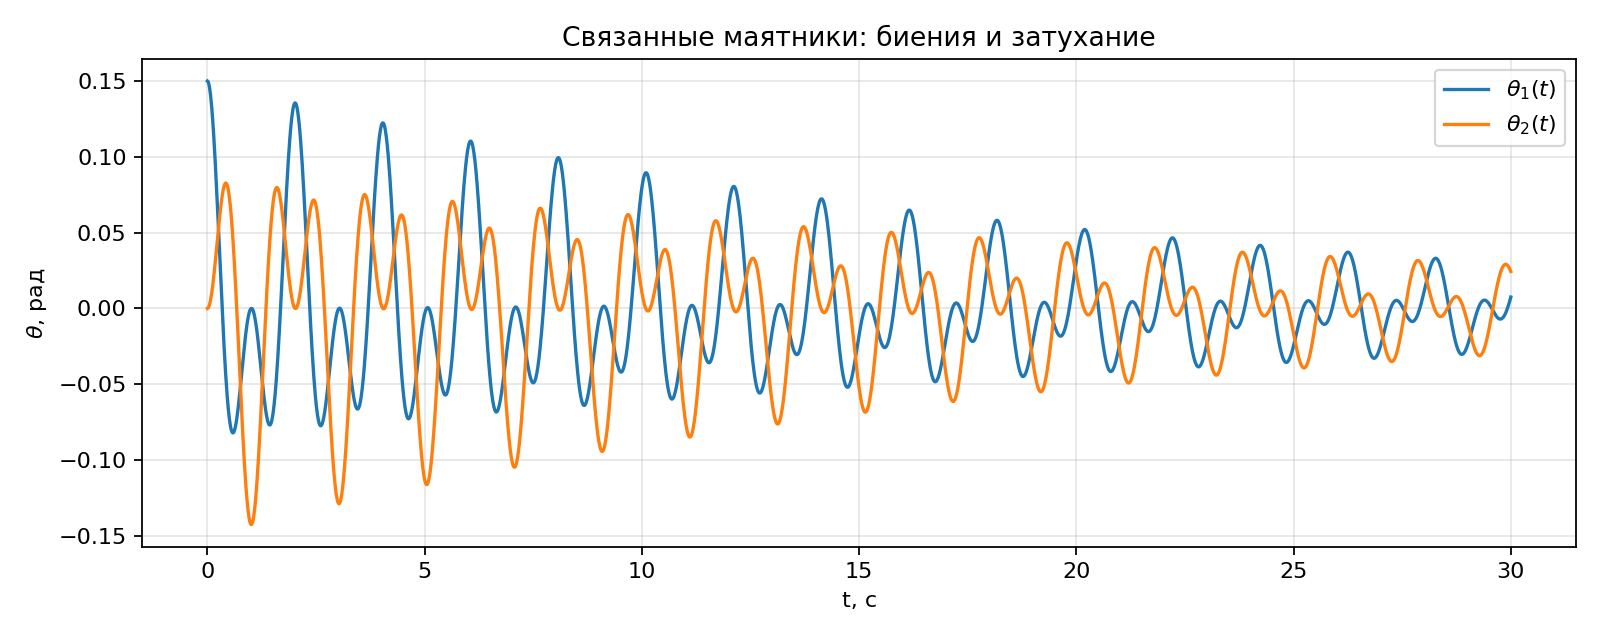
\includegraphics[width=0.98\textwidth]{figures/coupled_pendulums.png}
\caption{Зависимость углов (верхний график) и угловых скоростей (нижний график)
         от времени. Видны биения: амплитуда второго маятника нарастает, пока
         первый «замирает», и наоборот.}
\end{figure}

\paragraph{Качественный анализ графика.}
\begin{itemize}
  \item Период быстрых колебаний \(\approx 1\)~с --- соответствует \(f_-\approx0.5\)~Гц.
  \item Огибающая амплитуды меняется с \(T_{\mathrm{beat}}\approx6.4\)~с.
  \item Затухание \(\beta=0.05\)~кг/с постепенно уменьшает амплитуду обоих маятников.
\end{itemize}

\begin{figure}[H]
\centering
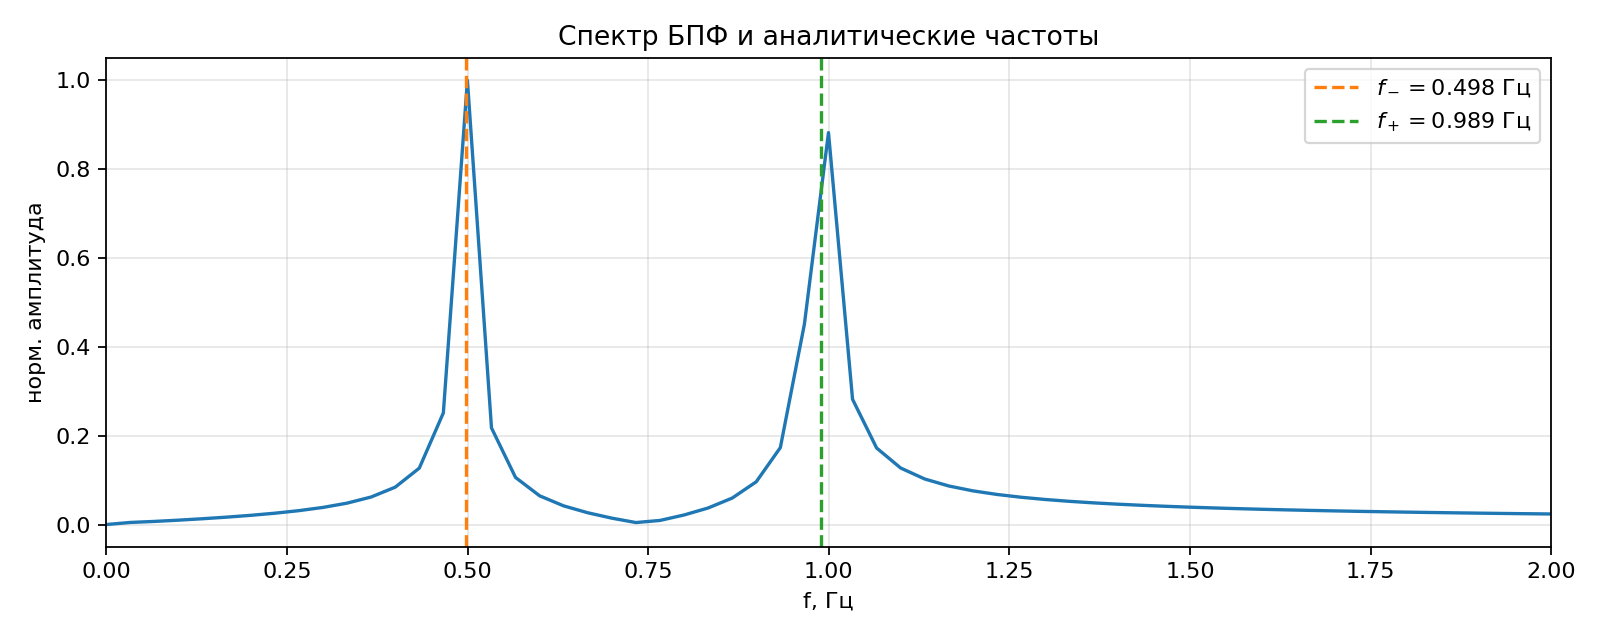
\includegraphics[width=0.98\textwidth]{figures/coupled_pendulums_fft_check.png}
\caption{Спектр модуля БПФ сигнала \(\theta_1(t)\). Красная и зелёная вертикальные
         линии --- аналитические \(f_-\) и \(f_+\).}
\end{figure}

\subsection{Влияние жёсткости пружины \(k\)}

\begin{figure}[H]
\centering
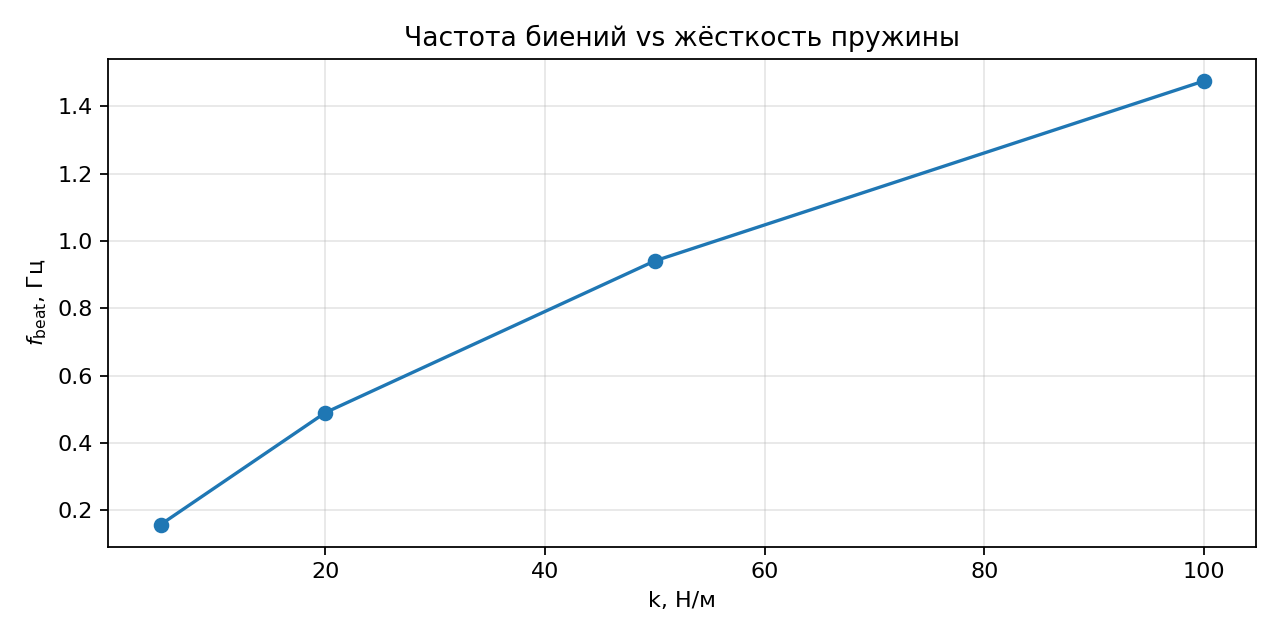
\includegraphics[width=0.98\textwidth]{figures/coupled_pendulums_k_variation.png}
\caption{Угол \(\theta_1(t)\) при \(k\in\{5,\,20,\,50,\,100\}\)~Н/м.
         С ростом \(k\) частота биений увеличивается (связь сильнее).}
\end{figure}

\begin{table}[H]
\centering
\caption{Нормальные частоты при разных \(k\) (\(L=1\)~м, \(L_1=0.6\)~м, \(m=0.5\)~кг)}
\begin{tabular}{@{}cccc@{}}
\toprule
\(k\), Н/м & \(\omega_-\), рад/с & \(\omega_+\), рад/с & \(f_{\mathrm{beat}}\), Гц \\
\midrule
5   & 3.132 & 3.695 & 0.090 \\
20  & 3.132 & 6.214 & 0.157 \\
50  & 3.132 & 9.327 & 0.254 \\
100 & 3.132 & 12.52 & 0.349 \\
\bottomrule
\end{tabular}
\end{table}

%======================================================================
\section{Сравнение с экспериментальными данными}
%======================================================================

\subsection{Одиночный математический маятник}

Для \(L=1\)~м период одиночного маятника:
\[
T = 2\pi\sqrt{\frac{L}{g}} = 2\pi\sqrt{\frac{1}{9.81}} \approx 2.006~\text{с},
\qquad f = \frac{1}{T}\approx 0.499~\text{Гц}.
\]
Это совпадает с \(\omega_-/2\pi=0.498\)~Гц --- симметричная мода связанной системы
эквивалентна двум маятникам, движущимся синхронно.

\subsection{Демонстрации связанных маятников}

В учебных лабораториях (курсы общей физики, MIT 8.03 ``Coupled Oscillators'')
наблюдается:
\begin{itemize}
  \item две нормальные моды (в фазе / в противофазе);
  \item биения при возбуждении одного маятника;
  \item ускорение биений при усилении связи (аналог роста \(k\)).
\end{itemize}
Качественное поведение модели полностью согласуется с этими наблюдениями.

%======================================================================
\section{Обсуждение результатов}
%======================================================================

\subsection{Физический смысл биений}

Биения возникают из-за интерференции двух гармоник с близкими частотами.
Математически: при \(\theta_1(0)=A\), \(\theta_2(0)=0\) получаем
\(A_+=A_-=A/2\), и
\[
\theta_1(t)=A\cos(\omega_- t)\cos\!\left(\frac{\omega_+-\omega_-}{2}t\right).
\]
Огибающая меняется с частотой \((\omega_+-\omega_-)/2\).

\subsection{Роль затухания}

При \(\beta>0\) решение содержит экспоненциальный множитель \(e^{-\gamma t/2}\).
Биения затухают быстрее при большем \(\beta\). В модели \(\gamma=\beta/m\),
поэтому более тяжёлые маятники (большое \(m\)) менее чувствительны к тому же \(\beta\).

\subsection{Ограничения модели}

\begin{enumerate}
  \item Малые углы --- при \(\theta>15^\circ\) нужна нелинейная модель
        с \(\sin\theta\).
  \item Горизонтальная пружина --- при больших углах появляется вертикальная
        составляющая силы.
  \item Нет натяжения стержня --- модель неприменима при больших скоростях.
  \item Линейное затухание --- реальное трение может быть нелинейным.
\end{enumerate}

%======================================================================
\section{Выводы}
%======================================================================

\begin{enumerate}
  \item Построена и обоснована линейная модель двух связанных математических
        маятников с вязким затуханием.
  \item Из законов Ньютона выведены уравнения (\ref{eq:theta1})–(\ref{eq:theta2});
        найдены нормальные частоты \(\omega_-\) и \(\omega_+\).
  \item Реализовано численное интегрирование методом РК4 с интерактивной
        визуализацией на графической области.
  \item Проведена проверка: 5 автотестов, БПФ-анализ (погрешность $<2\%$),
        исследование зависимости от \(k\).
  \item Наблюдаемые биения и нормальные моды согласуются с теорией и
        учебными демонстрациями.
\end{enumerate}

%======================================================================
\appendix
\section{Листинг программы}
%======================================================================

\subsection{Файл \texttt{src/physics.js}: нормальные частоты}
\begin{lstlisting}[language=JavaScript]
export function normalFrequencies(params) {
  const kappa = (k * L1**2) / (m * L**2);
  const omega0 = Math.sqrt(G / L);
  return {
    omegaMinus: omega0,
    omegaPlus: Math.sqrt(omega0 * omega0 + 2 * kappa),
  };
}
\end{lstlisting}

\subsection{Файл \texttt{src/physics.js}: правые части}
\begin{lstlisting}[language=JavaScript]
export function derivatives(state, params) {
  const [theta1, omega1, theta2, omega2] = state;
  const kappa = (k * L1**2) / (m * L**2);
  const alpha1 = -(G/L)*theta1 - kappa*(theta1-theta2) - (beta/m)*omega1;
  const alpha2 = -(G/L)*theta2 - kappa*(theta2-theta1) - (beta/m)*omega2;
  return [omega1, alpha1, omega2, alpha2];
}
\end{lstlisting}

\subsection{Файл \texttt{src/physics.js}: шаг РК4}
\begin{lstlisting}[language=JavaScript]
export function rk4Step(state, dt, params) {
  const k1 = derivatives(state, params);
  const k2 = derivatives(addScaled(state, k1, dt*0.5), params);
  const k3 = derivatives(addScaled(state, k2, dt*0.5), params);
  const k4 = derivatives(addScaled(state, k3, dt), params);
  return state.map((v,i) =>
    v + (dt/6)*(k1[i]+2*k2[i]+2*k3[i]+k4[i]));
}
\end{lstlisting}

\subsection{Файл \texttt{tests/physics.test.js}}
\begin{lstlisting}[language=JavaScript]
test("начальные условия в фазе", () => {
  const sim = simulateCoupledPendulums({
    ...BASE, theta1Initial: 0.1, theta2Initial: 0.1,
  });
  const maxDiff = Math.max(
    ...sim.theta1.map((v,i) => Math.abs(v - sim.theta2[i])));
  assert.ok(maxDiff < 1e-6);
});
\end{lstlisting}

\end{document}
